\chapter{Data}
\label{ch:data}

\section{FLAMINGO}
The main data used is the FLAMINGO (Full-hydro Large-scale structure simulations with All-sky Mapping for the Interpretation of Next Generation Observations) simulations, see also \citet{schaye2023, kugel2023}. The FLAMINGO simulations are large-scale hydrodynamical simulations, that explicitly incorporate baryonic physics. The aim of these simulations is to provide more accurate theoretical predictions for observational cosmology, particularly on smaller scales where baryonic effects become more dominant and complex. \par 
The FLAMINGO data we used contains an initial distribution of particles, and eight subsequent evolutionary timestamps. In general, information includes the scale factor and redshifts. Then, for each timestamp, information about the particle locations, types and masses are given. \par 
We used a dark-matter only simulation, with a box size of $400$ Mpc and $360^3$ particles. A projection of the cold dark matter surface density can be found in Figure~\ref{fig:cdmdensity}. Some denser and less-dense structures can be seen, as we would expect in the Cosmic Web. The data was processed with \lstinline|swiftsimio| \citep{swiftsimio}. Besides the FLAMINGO data, we have generated data for specific patterns of motion, which will be elaborated in Chapter~\ref{ch:results}. 

\begin{figure}[!ht]
	\centering 
	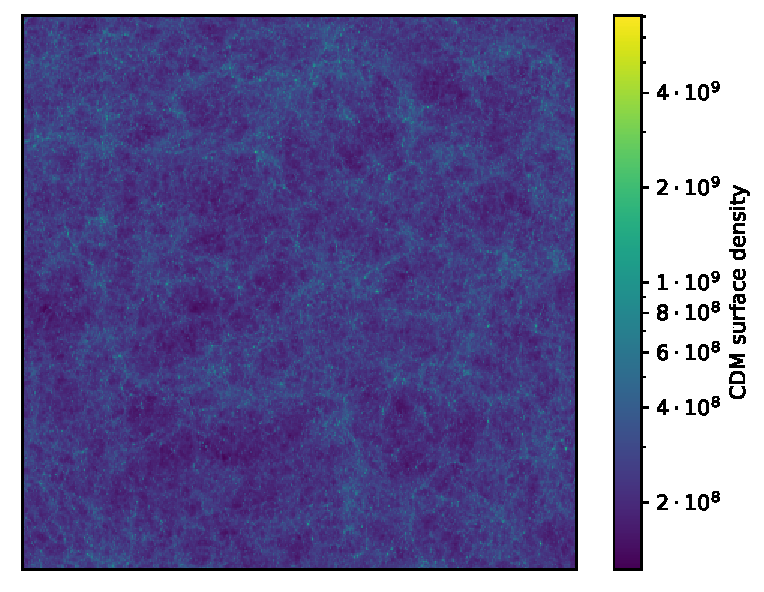
\includegraphics[width=8cm]{./images/projection.pdf}
	\caption{Cold Dark Matter (CDM) surface density of the used FLAMINGO simulation; a dark-matter only simulation with a box size of $400$ Mpc and $360^3$ particles.}
	\label{fig:cdmdensity}
\end{figure}

\subsection{Boxes}
\label{sec:boxes}
As the simulations have about 50 million particles for each time-step, evaluating each particle can be computationally expensive. To not look into each particle separately, the data is divided into $n^3$ boxes of equal size - each axis is divided into $n$ parts. The boxes are counted in the following way: box $0$ is the box around $(0, 0, 0)$. Then, taking the same $x$ and $y$, we will count the boxes upward in $z$. Once we have reached the maximum $z$-value, we will move up one $y$-segment, and again count up in $z$. We repeat this until there are no more $y$-segments. Once this is the case, we move up one $x$-segment, and repeat this process. We stop once all the $x$-values have been covered, resulting in $n^3$ boxes. The $n=2$ case can be seen in Figure~\ref{fig:boxes}. Note that we implicitly assume here, that there are no negative coordinates. \par %This is always the case in the simulations always the case, and other situations can always be translated into this case. \par
\begin{figure}[!ht]
	\centering
	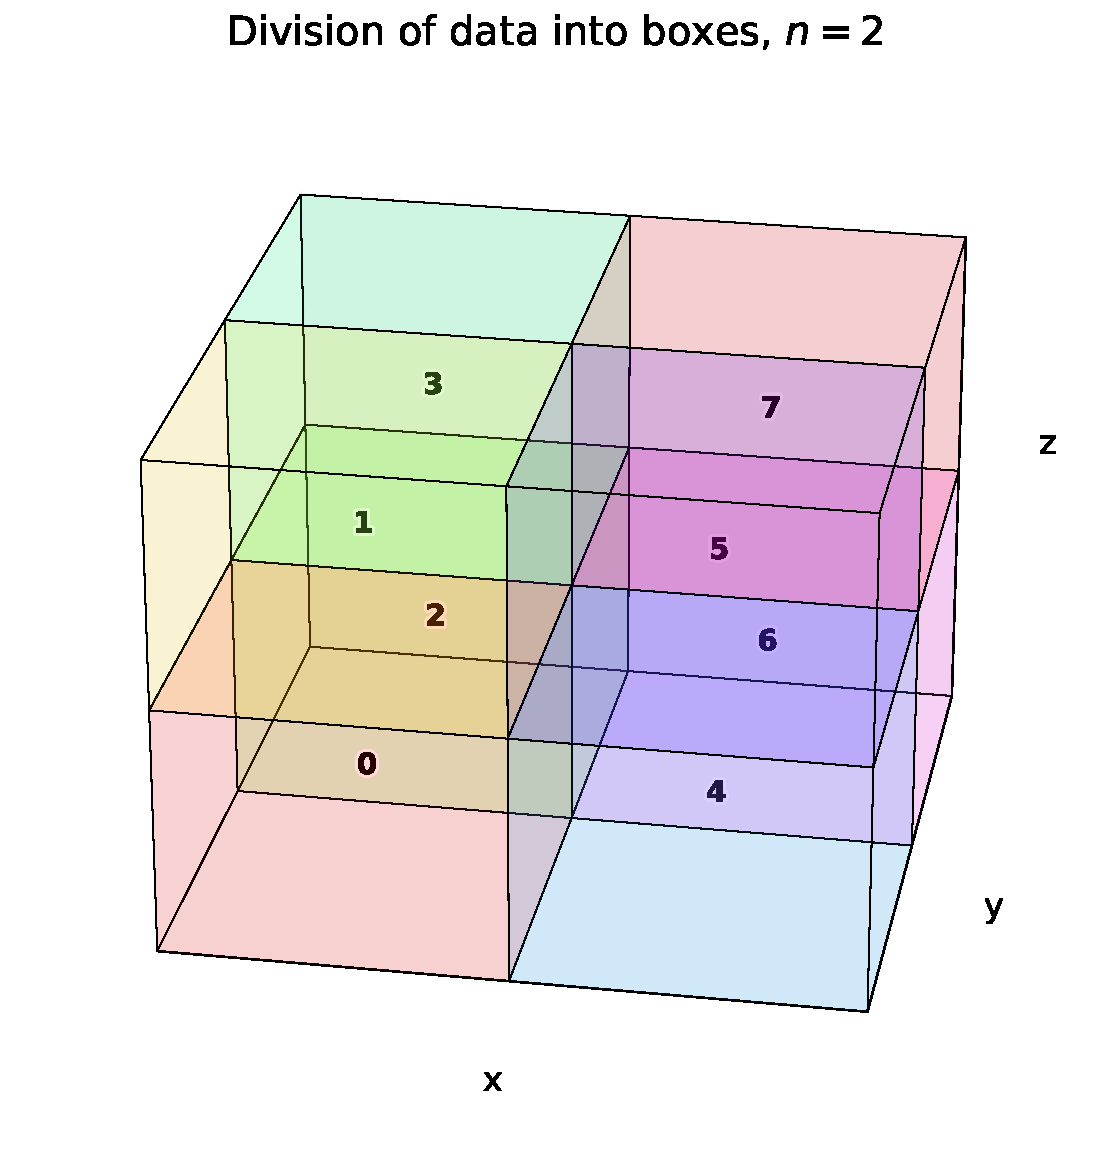
\includegraphics[width=8cm]{./images/boxes.pdf}
	\caption{Division of the data into boxes, for the case $n=2$. }
	\label{fig:boxes}
\end{figure}


By dividing the data into boxes, the cost matrix will be a function of these boxes, and not of the specific particles. Therefore, the cost matrix depends on the amount of particles in each box and the dynamics of those particles on average, rather then the dynamics of the individual particles. 




